
\documentclass[hidelinks, a4paper,11pt]{article}
\usepackage{csquotes}
\usepackage{marvosym}
\usepackage[a4paper,bottom=1.5in,right=1in,left=1in,top=42mm]{geometry}
\usepackage[fleqn]{mathtools}
\usepackage{graphicx}
\usepackage{hyperref}
\usepackage{colortbl}
\usepackage{tikz} %Drawing Graph
\usepackage[edges]{forest} %Drawing Tree

\usepackage{longtable}

\usepackage{course}
\usepackage{color}
\usepackage{hyperref}
\usepackage{fontspec}
\settextfont[Scale=1]{XB Niloofar}
%\setlatintextfont[Scale=0.9]{Tahoma}
\lstset{language=C}
\newcommand\tab[1][1cm]{\hspace*{#1}}
\definecolor{sepgray}{gray}{0.8}

\usetikzlibrary{positioning}

\newcolumntype{C}[1]{>{\centering\arraybackslash}m{#1}}



\begin{document}


\سربرگ{امتحان پایان‌ترم}{\lr{}}{مصطفی قدیمی}


\فصل{مفهوم تست خودکار}

در این فصل نکات کلی و برخی مفاهیم در خودکارسازی فرآیند تست نرم‌افزار به اختصار توضیح داده می‌شود.

\قسمت{‌خودکارسازی تست چیست؟}

مفهوم فرآیند خودکارسازی تست‌ها به استفاده از ابزارهای خاصی برای کنترل اجرای تست‌ها و مقایسه‌ی نتایج آن‌ها با نتایج مورد انتظار می‌گویند. ابزارهای تست نه‌تنها به ما کمک می‌کنند تا تست‌های رگرسیون را انجام دهیم، بلکه کمک می‌کند تا تولید داده‌ها، نصب محصول، تعامل با رابط گرافیکی و... خودکار شود.

\قسمت{ملاک‌های انتخاب ابزار}
برای خودکارسازی هر برنامه‌ای، باید به موارد زیر توجه کنیم:



\شروع{فقرات}

\فقره قابلیت داده‌محور بودن
\فقره عدم وابستگی به پلتفرم
\فقره قابلیت اجراپذیری و شخصی‌سازی
\فقره اعلان ایمیل
\فقره قابلیت استفاده از \lr{ٰVersion Control}
\فقره قابلیت عیب‌یابی و \lr{logging}
\فقره و...
\پایان{فقرات}

\قسمت{انواع چارچوب‌ها}

به طور معمول، چهار چارچوب خودکارسازی تست وجود دارد که در حین خودکارسازی برنامه‌ها انتخاب می‌شوند:

\شروع{فقرات}

\فقره چارچوب خودکارسازی داده‌محور
\فقره چارچوب خودکارسازی کلیدواژه‌محور
\فقره چارجوب خودکارسازی ماژولار
\فقره چارچوب خودکارسازی ترکیبی

\پایان{فقرات}


\قسمت{تست کیس}

تست کیس یک سندی است که دارای مجموعه‌ای از داده‌های تست، پیش‌شرط‌ها، نتایج مورد انتظار و پس‌شرط‌ها است که برای یک سناریو تست مشخص طراحی شده تا یک نیاز مشخص را تایید و اعتبارسنجی کند.

\قسمت{طراحی تست‌ کیس}

در قسمت زیر، تکنیک‌های متداول طراحی تست کیس در مهندسی نرم‌افزار آورده شده است.

\شروع{شمارش}
\فقره استخراج تست کیس‌ها به‌طور مستقیم از نیازمندی‌های تعریف شده یا تکنیک طراحی جعبه سیاه. این تکنیک شامل:
	\شروع{فقرات}
	\فقره تجزیه و تجلیل مرز مقادیر
	\فقره افراز به قسمت‌های برابر
	\فقره جدول تصمیم‌گیری تست
	\فقره نمودار انتقال حالت
	\فقره تست موارد استفاده
	\پایان{فقرات}
است.



\فقره استخراج تست کیس‌ها به طور مستقیم از ساختار یک جزء یا سیستم.
\شروع{فقرات}
\فقره پوشش \lr{Statement}
\فقره پوشش \lr{Branch}
\فقره پوشش \lr{Path}
\فقره تست \lr{LCSAJ}
\پایان{فقرات}

 \فقره استخراج تست کیس‌ها براساس تجربه‌ی آزمون‌گر روی سیستم‌های مشابه یا شهود.

\شروع{فقرات}
\فقره خطا در حدس‌زدن
\فقره تست اکتشافی
\پایان{فقرات}
\پایان{شمارش}

\newpage
\فصل{پیاده‌سازی تست خودکار}

در این فصل به نحوه‌ی پیاده‌سازی تست خودکار می‌پردازیم. 

\قسمت{جامعیت تست خودکار}

موقع ارزیابی یک راه‌حل تست، داشتن یک ابزار که مناسب نیاز‌های همه‌ی اعضای تیم فرآیند تست، بسیار ضروری است. این افراد عبارتند از:

\شروع{فقرات}
\فقره \مهم{آزمون‌گرهای دستی}:‌ ضبط و اجرای دوباره یک کار حیاتی برای آزمون‌گرهای دستی است. مخصوصأ آن دسته که در تست خودکار تازه‌کار هستند. توانایی استفاده از اسکریپت‌های ضبط شده یکسان با داده‌های مختلف می‌تواند به صورت دستی حین شناسایی و رفع مشکلات از طریق چندین محیط انجام شود.

\فقره \مهم{مهندسان خودکارسازی}: برای مهندسان خودکارسازی، پشتیبانی قدرتمند از زبان‌های اسکریپت‌نویسی، ادغام با سیستم‌های \lr{CI} و توانایی مقیاس‌پذیر کردن تست‌ها می‌تواند مهم باشد.
\فقره \مهم{توسعه‌دهندگان}: پیاده‌سازی تست‌ها در فرآیند توسعه نیازمند توانایی برای انجام دادن تست‌ها درون \lr{IDE}های مختلف نظیر \lr{Visual Studio Code}
\پایان{فقرات}

\قسمت{تصورهای غلط رایج مربوط به تست خودکار}

\شروع{شمارش}
\فقره \مهم{خودکارسازی وقت آزاد بیش‌تری فراهم می‌کند.}
\\
این تصور که تست خودکار وقت آزاد بیش‌تری به ما می‌دهد هم درست است و هم غلط.
در تست دستی، بیش‌تر زمان برای اکتشاف و تست کردن کارایی اختصاص می‌یابد که باید به طور دستی به دنبال خطاها بگردیم. یک‌بار که این کار انجام می‌شود، آزمون‌گر دستی باید مکررأ این کارها را اجرا کند. اما استفاده از تست خودکار باعث می‌شود که این زمان به شدت کاهش یابد. کار آزمون‌گرهای تست خودکار این است که زمان‌شان را صرف کد زدن تست‌ها و اعمال بهبود روی آن تست‌ها به صورت مکرر است. در اصل، زمان صرف‌شده برای کارهای روزمره و تکراری آزمون‌گر دستی برای آزمون‌گر خودکار صرف تمرکز روی موضوعات بزرگ‌تر و مهم‌تری که شامل نرم‌افزار در حال توسعه می‌شود، می‌باشد.

\فقره \مهم{هزینه‌ی تست خودکار بسیار بالا است.}
\\
در ابتدا، سرمایه‌گذاری روی تست اتوماتیک ممکن است هزینه‌بر به نظر برسد، به خصوص اگر صاحب یک شرکت کوچک باشیم. اما تحلیل‌ها نشان داده است که با گذشت زمان، تست خودکار هزینه‌ی خودش را می‌پردازد (هزینه‌ی اضافی ندارد). همان‌طور که قبلا اشاره شد، تست اتوماتیک شما را آزادتر می‌کند تا بتوانید روی مسائل مهم‌تر مانند نیاز‌های مشتری، کارایی و بهبودها تمرکزکنید. هم‌چنین تست خودکار هزینه‌ها و نیاز به بازبینی برنامه را کاهش می‌دهد. علاوه‌براین هر بار که منبع کد تغییر پیدا می‌کند، تست‌های نرم‌افزار می‌تواند تکرار شود. تکرار این تست‌ها به صورت دستی هزینه‌بر است و زمان زیادی را مصرف می‌کند اما تست خودکار می‌تواند بدون هزینه‌ی اضافی تکرار شود.

\فقره \مهم{تست اتوماتیک بهتر از تست دستی است.}
\\
واقعیت این است که بهتر و بدتری وجود ندارد. هر کدام از راه‌کارها خوبی‌ها و بدی‌های خودشان را دارند. تست دستی توسط یک نفر که جلوی کامپیوتر نشسته است به کمک بررسی دقیق \lr{log}هاُ، تلاش برای دادن ورودی‌های مختلف، مقایسه‌ی نتیجه با رفتار مورد انتظار و ضبط نتایج انجام می‌شود.  این در حالی است که تست خودکار معمولأ وقتی نسخه‌ی اولیه‌ی نرم‌افزار توسعه داده شده است، انجام می‌گیرد. 

\فقره  \مهم{تست خودکار از تعامل انسانی جلوگیری می‌کند.}
\\
یکیدیگر از تصورهای غلط درباره تست خودکار این است که تعامل انسانی را تضعیف می‌کند. به طور دقیق‌تر، تست‌های اتوماتیک سریع‌تر از توانایی انسان می‌تواند آزمایش‌ها را انجام دهد با این مزیت که بدون خطای انسانی است.  . بنابراین این تصور قابل درک است. 
\\
البته این موضوع جایگزین روابط چهره به چهره و ملاقاتی که برای قسمت‌های توسعه نرم‌افزار ضروری است، نمی‌باشد. در عوض، با ارائه‌ی یک کانال دیگر ارتباطی، این جنبه را بهبود می‌بخشد. برای مثال ایمیل جای‌گزین تلفن نشد و صرفا یک ابزار اضافی برای برقراری ارتباط بود.

\پایان{شمارش}

\قسمت{تشریح چارچوب‌های تست خودکار}

\شروع{شمارش}

	\فقره \مهم{چارچوب خودکارسازی داده‌محور}
	\شروع{فقرات}
	\فقره 
	\textbf{تعریف} 
	با استفاده از چارچوب داده محور، داده‌های تست را از منطق اسکریپت جدا می‌شوند، به این معنی که مهندسان تست می‌توانند داده‌ها را در یک منبع جدا ذخیره کنند. خیلی اوقات، مهندسان تست در شرایطی قرار می‌گیرند که باید چندین بار ویژگی‌ها یا عمل‌کردهای یک برنامه را با مجموعه‌های مختلف داده تست کنند. در این موارد، بسیار مهم است که داده‌های آزمون در خود اسکریپت \lr{hard-code} نباشند، این اتفاقی است که با یک چارچوب تست خطی یا مبتنی بر ماژولار رخ می‌دهد.
	
	تنظیم چارچوب تست داده‌محور به مهندسان تست این امکان را می‌دهد تا پارامترهای ورودی/خروجی را آزمایش کند و اسکریپت‌ها را از یک منبع داده خارجی مانند \lr{Excel Spreadsheets}، \lr{Text Files}، \lr{CSV}، جداول  \lr{SQL} یا مخازن \lr{ODBC} ذخیره کند.
	
	اسکریپت‌های تست به منبع داده خارجی متصل شده و در صورت لزوم داده‌های لازم را می‌خوانند.
	
	
	\فقره 
	\textbf{مزایا} 
	تست‌ها را می‌توان با مجموعه داده‌های متعدد اجرا کرد.
	
	با تغییر داده‌ها می‌توان به سرعت چندین سناریو را آزمایش کرد و از این طریق تعداد اسکریپت‌های مورد نیاز را کاهش داد.
	
	از \lr{hard-code} کردن داده‌ها می‌توان جلوگیری کرد بنابراین هرگونه تغییر در اسکریپت‌های آزمایشی روی داده‌های مورد استفاده تاثیر نمی‌گذارد و برعکس.
	
	با اجرای سریع‌تر تست‌های بیش‌تر، در وقت صرفه‌جویی می‌شود.
	
	
	\فقره
	\textbf{معایب}
	
	برای استفاده صحیح از این چارچوب، به یک مهندس تست باتجربه و دارای مهارت در زبان‌های مختلف برنامه‌نویسی نیاز دارید. آن‌ها باید منابع داده خارجی را شناسایی و قالب‌بندی کنند و کدی را بنویسند (ایجاد توابع) که آزمایش‌ها را به صورت یک‌پارچه به منابع داده خارجی متصل می‌کند.
	
	تنظیم یک چارچوب داده‌محور زمان زیادی را می‌طلبد.

	
	\پایان{فقرات}
	
	\فقره \مهم{چارچوب خودکارسازی کلیدواژه‌محور}
	\شروع{فقرات}
	\فقره 
	\textbf{تعریف}
	در یک چارچوب کلید‌واژه‌محور‌، هر عمل‌کرد برنامه مورد تست در یک جدول با یک سری دستورالعمل به ترتیب متوالی برای هر تست که باید اجرا شود، قرار داده شده است. با روشی مشابه چارچوب داده محور، داده‌های تست و منطق اسکریپت در یک چارچوب کلیدواژه‌محور از هم جدا می‌شوند، اما این رویکرد آن را یک قدم فراتر می‌برد.
	
	با این رویکرد، کلمات کلیدی نیز در یک جدول داده خارجی ذخیره می‌شوند و باعث می‌شوند که آن‌ها از ابزار تست خودکار که برای اجرای تست‌ها استفاده می‌شود، مستقل شوند. کلمات کلیدی بخشی از یک اسکریپت است که نمایان‌گر اقدامات مختلفی است که برای تست \lr{GUI} یک برنامه انجام می‌شود. این موارد می‌توانند به سادگی با \lr{"click"}، یا \lr{"login"} یا برچسب‌های پیچیده مانند \lr{"clicklink"}، یا \lr{"verifylink"} برچسب‌گذاری شوند.
	
	در جدول، کلمات کلیدی به صورت مرحله به مرحله با یک آبجکت مرتبط یا بخشی از رابط کاربری که عمل در آن انجام می‌شود، ذخیره می‌شوند. برای این‌که این روی‌کرد به درستی کار کند، یک مخزن آبجکت مشترک برای یافتن اقدامات مرتبط با هر آبجکت لازم است.
	
	جدول
	
	
	
	\فقره
	\textbf{مزایا}
	دانش برنامه‌نویسی حداقل مورد نیاز است.
	
	یک کلمه کلیدی واحد را می‌توان در چندین اسکریپت تست استفاده کرد‌، بنابراین کد قابل استفاده مجدد است.
	
	اسکریپت تست را می‌توان مستقل از نرم‌افزار تحت آزمون ساخته شده است.
	
	\فقره
	\textbf{معایب}
		هزینه اولیه تنظیم چارچوب زیاد است. وقتٰگیر و پیچیده است. کلمات کلیدی نیاز به تعریف دارند و باید مخازن/کتاب‌خانه‌های آبجکت تنظیم شود.
	
	شما به یک مهندس تست با مهارت‌های اتوماسیون بالا نیاز دارید.
	
	هنگام مقیاس دادن به عملیات تست، کلمات کلیدی می‌توانند به دردسر تبدیل شوند. شما نیاز به ادامه ساخت مخازن و جداول کلمات کلیدی دارید.
	
	\پایان{فقرات}
	
	\فقره \مهم{چارجوب خودکارسازی ماژولار}
	
	\شروع{فقرات}
	\فقره 
	\textbf{تعریف} 
	اجرای یک چارچوب ماژولار به مهندسین تست نیاز دارد تا برنامه مورد آزمایش را به واحدها ، کارکردها یا بخش‌های جداگانه تقسیم کنند که هر یک از آن‌ها به صورت جداگانه تست می‌شوند. پس از شکستن برنامه به ماژول‌های جداگانه، یک اسکریپت تست برای هر قسمت ایجاد می‌شود و سپس برای ساخت تست‌های بزرگ‌تر به صورت سلسله مراتبی ترکیب می‌شود. این مجموعه‌های تست بزرگ‌تر شروع به نمایش تست کیس‌ها می‌کنند.
	
	یک استراتژی اساسی در استفاده از چارچوب ماژولار ایجاد یک لایه انتزاع است، به طوری که هرگونه تغییر در بخش‌های خاص بر ماژول اصلی تاثیر نمی‌گذارد.
	
	
	\فقره 
	\textbf{مزایا} 
	در صورت ایجاد هرگونه تغییر در برنامه، فقط باید ماژول و آن اسکریپت تست مرتبط با آن تغییر یابد، به این معنی که لازم نیست بقیه تست‌ها را تغییر دهید و می‌توانید آن‌ها را دست نخورده بگذارید.
	
	ایجاد موارد آزمایشی تلاش کم‌تری می‌کند زیرا می‌توان از اسکریپت‌های آزمون برای ماژول‌های مختلف استفاده مجدد کرد.
	\فقره
	\textbf{معایب}
	داده‌ها از آن‌جا که تست‌ها به طور جداگانه انجام می‌شوند  به صورت \lr{hard-code} در تست‌ها قرار دارند، بنابراین نمی‌توانید از چندین مجموعه داده استفاده کنید.
	
	دانش برنامه نویسی برای تنظیم این چارچوب نیاز است.
	
	
	\پایان{فقرات}

	
	\فقره \مهم{چارچوب خودکارسازی ترکیبی}

	\شروع{فقرات}
\فقره 
\textbf{تعریف}
مانند اکثر فرایندهای تست امروز، چارچوب‌های تست خودکار شروع به یک‌پارچه‌سازی و هم‌پوشانی با یک‌دیگر می‌کنند. یک چارچوب ترکیبی، ترکیبی از هر یک از چارچوب‌های قبلی است که برای استفاده از مزایای برخی و کاهش نقاط ضعف برخی دیگر تنظیم شده است.

هر برنامه متفاوت است، بنابراین باید فرآیندهای تست آن‌ها نیز متفاوت باشد. با حرکت تیم‌های بیش‌تر به یک مدل چابک ، تنظیم یک چارچوب انعطاف‌پذیر برای تست خودکار بسیار مهم است. یک چارچوب ترکیبی می‌تواند به آسانی با نیاز ما سازگار شود تا بهترین نتایج تست را به دست آوریم.

\پایان{فقرات}


\پایان{شمارش}
\newpage

\سؤال{}

\textbf{شرکت‌ها و به‌ویژه شرکت‌های نرم‌افزاری هم مانند انسان‌ها مراحل رشد و شکوفایی دارند. برای بررسی این بلوغ از روش‌هایی مانند \lr{CBA-IPI} که در فصل سوم کتاب مطرح شده، استفاده می‌شود. لطفا با انجام تحقیق کوچکی مراحل مختلف بلوغ سازمان‌ها را در این روش به اختصار مشخص کنید.}


سطح بلوغ یک تکامل خوش‌تعریف\footnote{well-defined} جهشی رو به جلو برای دست‌یابی به یک فرآیند نرم‌افزاری بالغ است. هر سطح بلوغ یک لایه‌ای را در پایه برای بهبود مداوم فرآیند فراهم می‌کند. 
\begin{figure}[!h]
	\begin{center}
		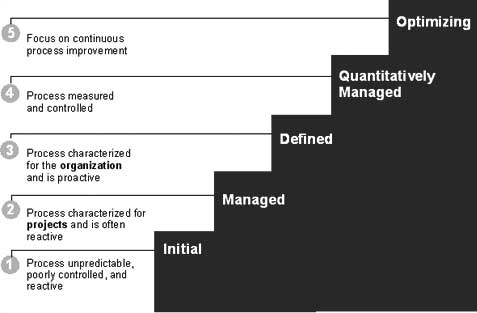
\includegraphics[scale=0.7]{./3.jpg}
	\end{center}
	\caption{مراحل بلوغ در سازمان‌ها}
\end{figure}

در مدل \lr{CMMI} \footnote{Capability Maturity Model Integration} از پنج سطح بلوغ تشکیل شده است:
\begin{enumerate}
	\item سطح اولیه\footnote{Initial}
	\item سطح مدیریت شده
	\item سطح تعریف شده
	\item سطح مدیریت شده از نظر کمّی\lr{Quantitatively Managed
	}
	\item سطح بهینه‌سازی
	
\end{enumerate}

حال هر سطح از سطوح بالا را به‌طور دقیق‌تر بررسی می‌کنیم:

\begin{itemize}
	\item 
	\textbf{سطح اولیه}
	
	در این سطح فرآیند‌ها معمولا نامشخص هستند. سازمان معمولا محیط پایداری را فراهم نمی‌کند و موفقیت در این سازمان‌ها ببیش‌تر ستگی به رقابت افراد و اعضای و نه استفاده از فرآیند‌های اثبات شده دارد. در این مرحله بعضی اوقات محصول یا سرویسی تولید می‌شود اما  قیمت تمام‌شده‌ی آن‌ها معمولا بالاتر از بودجه‌ی اختصاص داده شده است.
	\item 
	\textbf{سطح مدیریت شده}
	
	در این سطح سازمان به همه‌ی اهداف کلی و خاص رسیده است. به بیان دیگر، پروژه‌های سازمان تضمین کرده‌اند که نیازمندی‌ها مدیریت می‌شوند و هم‌چنین فرآیندها نیز برنامه‌ریزی، انجام، اندازه‌گیری و کنترل می‌شوند.
	
	در این مرحله تعهدات بین سهام‌داران ایجاد شده و در صورت نیاز مورد بازبینی و تجدید نظر قرار می‌گیرد.
	
	\item
	\textbf{سطح تعریف شده}
	
	در این سطح فرآیندها به خوبی مشخص و درک شده و در قالب استاندارد‌ها، رویه‌ها\footnote{procedure}، ابزارها و روش‌ها بیان می‌شوند.
	تفاوت اصلی و مهم بین سطح شماره‌ی «۳» و «۲» در محدوده استانداردها، توضیحات فرآیندها و رویه‌ها می‌باشد. در سطح «۲» استانداردها، توضیحات فرآیند و رویه‌ها ممکن است در هر نمونه خاص از فرآیند (مانند یک پروژه خاص) کاملا متفاوت باشند اما در مورد «۳» این تفاوت وجود ندارد و سازمان یک‌پارچه است.
	
	\item 
	\textbf{سطح مدیریت شده از نظر کمّی}
	
	در این سطح فرآیندهای فرعی که به‌طور قابل توجهی در عملکرد \footnote{performance}کلی فرآیند تاثیرگذارند، انتخاب می‌شوند. این فرآیندها با استفاده از روش‌های آماری و دیگر تکنیک‌های اندازه‌گیری کمّی کنترل می‌شوند. اهداف کمّی به عنوان معیاری برای مدیریت فرآیند‌ها ایجاد می‌شوند. این اهداف براساس نیازهای مشتری، کاربران نهایی\footnote{end users}، سازمان‌ها و مجریان فرآیند هستند.
	
	تفاوت اصلی این سطح با سطح شماره‌ی «۳» «قابلیت پیش‌بینی عمل‌کرد فرآیندها» است.
	
	\item 
	\textbf{بهینه‌سازی}
	
	در این سطح فرآیند‌ها به‌طور مداوم بر اساس درک کمّی از دلایل مشترک تغییر ذاتی فرآیند‌ها بهبود می‌یابند و بیش‌تر تمرکز آن بر روی پیشرفت ادامه‌پذیر عمل‌کرد فرآیند از طریق کارهای تکراری-افزایشی\footnote{iterative and incremental} است.
	
	این سطح در مقایسه با سطح «۴» در این مورد تفاوت دارند که در آن مشکلی  برای کافی بودن عوامل برای دست‌یابی به نتایج  اهداف وجود ندارد
\end{itemize}

\textbf{نکته} هر کدام از سطوح گفته شده ضروری هستند و نباید از آن‌ها پرش کرد.\footnote{skip} در صورت پرش کردن، هر چه سطح بالاتر باشد، احتمال رسیدن به موفقیت کم‌تر می‌شود.
\newpage
\سؤال{}

\textbf{\lr{Agile} مفهومی است که این روز‌ها در دنیای مهندسی نرم‌افزار خیلی مطرح می‌شود. شما با مفاهیمی مانند \lr{Scrum} و \lr{XP} در کلاس کمی آشنا شده‌اید. در شرکت‌هایی که از \lr{Scrum} استفاده می‌کنند، معمولا از ابزاری مانند \lr{tfs} برای مدیریت مراحل مختلف در فرآیند استفاده می‌شود. لطفا در خصوص این نرم‌افزار تحقیق کنید و نتایج آن را مختصرا گزارش دهید. تحقیقتان در حیطه مباحثی باشد که در کلاس مطرح شده است. یعنی ببینید موارد مطرح شده در کلاس در نرم‌افزار چگونه دیده شده است.}
\\
\\
\lr{TFS} یک ابزار مدیریت چرخه‌ی حیات نرم‌افزار \footnote{\lr{Application Lifecycle Management (ALM)}}است. 

در واقع \lr{TFS} مجموعه‌ای از ابزارهای مختلف تعاملی برای تولید نرم‌افزار را فراهم می‌کند که همه‌ی تیم ایجاد و توسعه نرم‌افزار از آن استفاده می‌کنند. این ابزارها شامل 
\begin{itemize}
	\item کنترل نسخه\footnote{\lr{version control}}
	\item ابزارهای گزارش‌دهی
	\item مدیریت نیازمندی‌ها
	\item مدیریت توزیع‌ها\footnote{\lr{release management}}
	\item و...

\end{itemize}
	است. به طور کلی با توجه به مطالب گفته شده می‌توان این نتیجه را گرفت که از آن می‌توان به عنوان یک \lr{backend} استفاده کرد. کاربرد اصلی آن در مستقرسازی\footnote{deployment} است که مفهومی به نام \lr{DevOps} در آن بسیار پررنگ است.
	
	\begin{figure}[!h]
		\begin{center}
			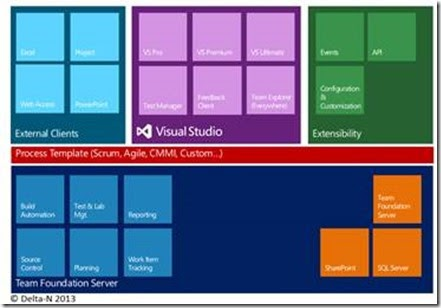
\includegraphics[scale=0.7]{./4.jpg}
		\end{center}
		\caption{نمای سطح بالای \lr{TFS}}
	\end{figure}

همان‌طور که در شکل شماره «۲» مشاهده ‌می‌شود (بدون پرداختن به هر جنبه به‌طور مستقل)، \lr{TFS} کاربردهای بسیار زیادی دارد و اساس بسیاری از موارد است. این اجازه را به ما می‌دهد تا منابع، مشکلات، برنامه‌ریزی و ساختن تست و... را به‌خوبی مدیریت کنیم. مهم‌ترین ویژگی \lr{TFS} توسعه‌پذیر \footnote{extensibility} آن است که آن را فوق‌العاده می‌کند؛ به این صورت که هر چیزی که وجود ندارد، یا می‌تواند ساخته شود و یا می‌تواند تغییر کند. این دقیقا همان چیزی است که استفاده از \lr{TFS} را برای سازمان‌ها مناسب می‌کند. ویژگی دیگر آن تنظیم‌پذیری \footnote{adjustability}و گستردگی آن است که هم می‌تواند تبدیل به نقطه قوت و هم نقطه ضعف آن شود؛ زیرا این ابزارها خاص منظوره هستند و عمل‌کرد آن‌ها باید بسته به کاربردشان  مقایسه و بررسی شود.


نحوه‌ی کار \lr{TFS} بدین صورت است که با \lr{process template}ها کار می‌کند. این قالب‌\footnote{template}ها از بخش‌های مختلفی شامل 
\begin{itemize}
	\item مورد کاری\footnote{\lr{work item}}
	\item گزارش‌ها
	\item مستندات
	\item نوع\footnote{type}‌ها
	\item و...
\end{itemize}
است و اجباری در انتخاب فرآیند انتخاب شده ندارد و دست مهندس نرم‌افزار را باز می‌گذارد.

\lr{TFS} می‌تواند در هر متدولوژی‌ای استفاده شود.  بسته به نوع متدولوژی‌ای که از آن استفاده می‌کنیم، مورد کاری تعریف می‌شود. این انعطاف‌پذیری زیاد باعث می‌شود که ساختار همه‌ی آن‌ها یکسان باشد.
\newpage
\سؤال{}

\textbf{تصور کنید که پس از اتمام تحصیل تصمیم به راه‌اندازی شرکتی نرم‌افزاری با دوستانتان گرفته‌اید. ساختار این شرکت از لحاظ نیروی انسانی به چه شکلی است؟ چه نیروهایی دارد؟ می‌توانید برای پاسخ‌گویی بهتر حوزه فعالیت شرکت را به دل‌خواه پیش‌نهاد دهید. مثلا بگویید شرکت بناست در حوزه تولید نرم‌افزارهای مالی فعالیت کند لذا این نیروها را خواهد خواست. }
\newline

\begin{itemize}
	\item الف)
	ساختار تیم نیروی انسانی به یکی از ۴ شکل زیر است: 
	\begin{enumerate}
		\item الگوی بسته \footnote{\lr{closed paradigm}}
		در این الگو، تیم به‌طور شکل سنتی و سلسله‌مراتبی دارد. این‌گونه تیم‌ها در هنگام تولید و ایجاد نرم‌افزار که شبیه کارهای گذشته باشد، به خوبی کار می‌کند. اما احتمال نوآورانه بودن آن در این الگوی بسته بسیار پایین است. 
		\item الگوی تصادفی \footnote{\lr{random paradigm}} د
		در این الگو یک تیم به نوآوری و  ابتکار فردی اعضای تیم وابستگی زیادی دارد. این الگو وقتی مزیت دارد که دست‌یابی به یک نوآوری یا موقعیت تکنولوژیکی مورد نیاز است. اما این متدولوژی هنگامی که عمل‌کرد منظم مطرح و ضروری می‌شود، عملکرد خوبی ندارد.
		\item الگوی باز\footnote{\lr{open paradigm}}
		در این الگو، سعی در ساختاربندی تیم به شکلی داریم که به برخی از کنترل‌های مرتبط با الگوی بسته دست یابد؛ هم‌چنین نوآوری‌های زیادی هنگام استفاده از الگوی تصادفی اتفاق می‌افتند. کارها با همکاری مشترک، ارتباطات سنگین و تصمیم‌گیری مبتنی بر تصمیم مشترک در مورد علائم تجاری تیم‌های با الگوی باز انجام می‌شود. ساختار تیم الگوی باز برای بسیاری از مسائل پیچیده مناسب است اما ممکن استبه اندازه سایر تیم‌ها کارآمد نباشد. 
		\item الگوی هماهنگ
		\footnote{\lr{synchronous paradigm}} 
		 این الگو متکی‌به تقسیم طبیعی یک مسئله است و اعضای تیم را برای داشتن ارتباط فعال با یک‌دیگر کمک می‌کند.
	\end{enumerate}
	\item در این سوال فرض می‌کنیم از متدولوژی چابک برای تشکیل روند تیم استفاده کنیم. استفاده از این متدولوژی باعث می‌شود تیم ساختار سلسله مراتبی داشته باشد و نقش‌ها در آن به شکل زیر است:
	\begin{figure}[!h]
		\begin{center}
			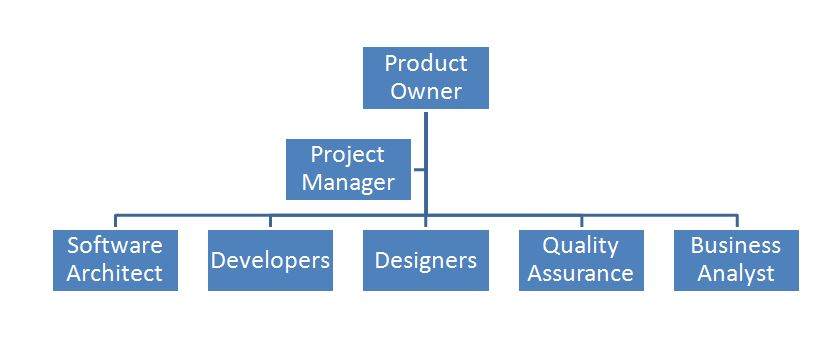
\includegraphics[width=\linewidth]{./5.jpg}
			\caption{ساختار تیم ایجاد و توسعه}
		\end{center}
	\end{figure}
	\item 
	در این سوال فرض شده است که می‌خواهیم یک سامانه حمل‌ونقل بار بین شهری ایجاد کنیم. به همین منظور در متدولوژی \lr{Agile}، نقش‌های مختلفی در تیم وجود دارد. برای مثال صاحب محصول\footnote{\lr{Product Owner }} همان مشتری است که با ما برای انجام پروژه در ارتباط است، محدودیت‌های مالی و زمانی را تعیین می‌کند و مطابق پروپوزال او، باید برنامه‌های تعیین نیازمندی‌های پروژه استخراج شود و سپس برنامه‌ی مدونی به او داده شود.
	
\end{itemize}
\end{document}
